% !TeX spellcheck = en_GB

\begin{frame}{$k\text{NN}$ and CART tuning}

\sideFigs{biasvar-knn-apple}{cp-tree-apple}

\end{frame}

% ------------------------------- %

%\begin{frame}[fragile]{Random forest}
%
%\begin{columns}[T]
%\begin{column}{0.7\textwidth}
%\begin{figure}
%\centering
%\hspace*{1em}\vspace*{-0.5em}%
%\begin{tikzpicture}
%	%draw,ellipse,fill=red!20,minimum height=2em,text centered,font=\sffamily\small
%	\tikzset{help lines/.append style=pink}
%	%	\draw [help lines] (-1,-4) grid (7,2); \node[draw,circle,fill=red] at (0,0) {};
%	
%	\node[cloud3] (b1) at (0,0) {$\pi_1, m_1$};
%	\node[cloud3] (b2) at ($(b1)+(1.8,0)$) {$\pi_2, m_2$};
%	\node[cloud3] (B) at ($(b2)+(3,0)$) {$\pi_B, m_B$};
%	\draw[-,dotted,very thick] (b1) to (b2);
%	\draw[-,dotted,very thick] (b2) to (B);
%	
%	\node[] (T1) at ($(b1)+(0,-1.3)$) {$T_1$};
%	\node[] (T2) at ($(b2)+(0,-1.3)$) {$T_2$};
%	\node[] (TB) at ($(B)+(0,-1.3)$) {$T_B$};
%	\draw[-stealth] ($(b1.south)+(0,-0.15)$) to (T1);
%	\draw[-stealth] ($(b2.south)+(0,-0.15)$) to (T2);
%	\draw[-stealth] ($(B.south)+(0,-0.15)$) to (TB);
%	
%	\begingroup\linespread{0.9}
%	\node[font=\footnotesize,text width=4em,centered,text centered,inner sep=0pt] (m) at (3.3,0.7) {random predictors};
%	\node[font=\footnotesize,text width=4em,centered,text centered,inner sep=0pt] (pi) at (3.1,-1.2) {random subsample};
%	\endgroup
%	\draw[-stealth] (m) to ($(b2.east)+(-0.2,0.1)$);
%	\draw[-stealth] (pi) to ($(b2.south)+(-0.1,0.25)$);
%	
%	\node[rectangle,fill=mLightGreen!20,font=\large,right] (G) at (-0.8,-3) {$G(x)=\argmax_k\sum_{b=1}^B\mathbb{I}(T_b(x)=k)$};
%	\node[rectangle,fill=red!20,font=\large,right] (mtry) at ($(G.west)+(0,-1)$) {$\mathtt{mtry}=\lfloor\sqrt{p}\rfloor$};
%\end{tikzpicture}
%\end{figure}
%\end{column}
%\hspace*{1em}\begin{column}{0.4\textwidth}
%\begin{lstlisting}
%randomForest(x, y,
%importance=TRUE,
%ntree=500,
%ntree=B.oob£!$\,\alert{\leftarrow}B^\ast$!£)
%\end{lstlisting}
%
%\vspace{1em}Loss-based variable importance
%
%%\hspace*{-0.8em}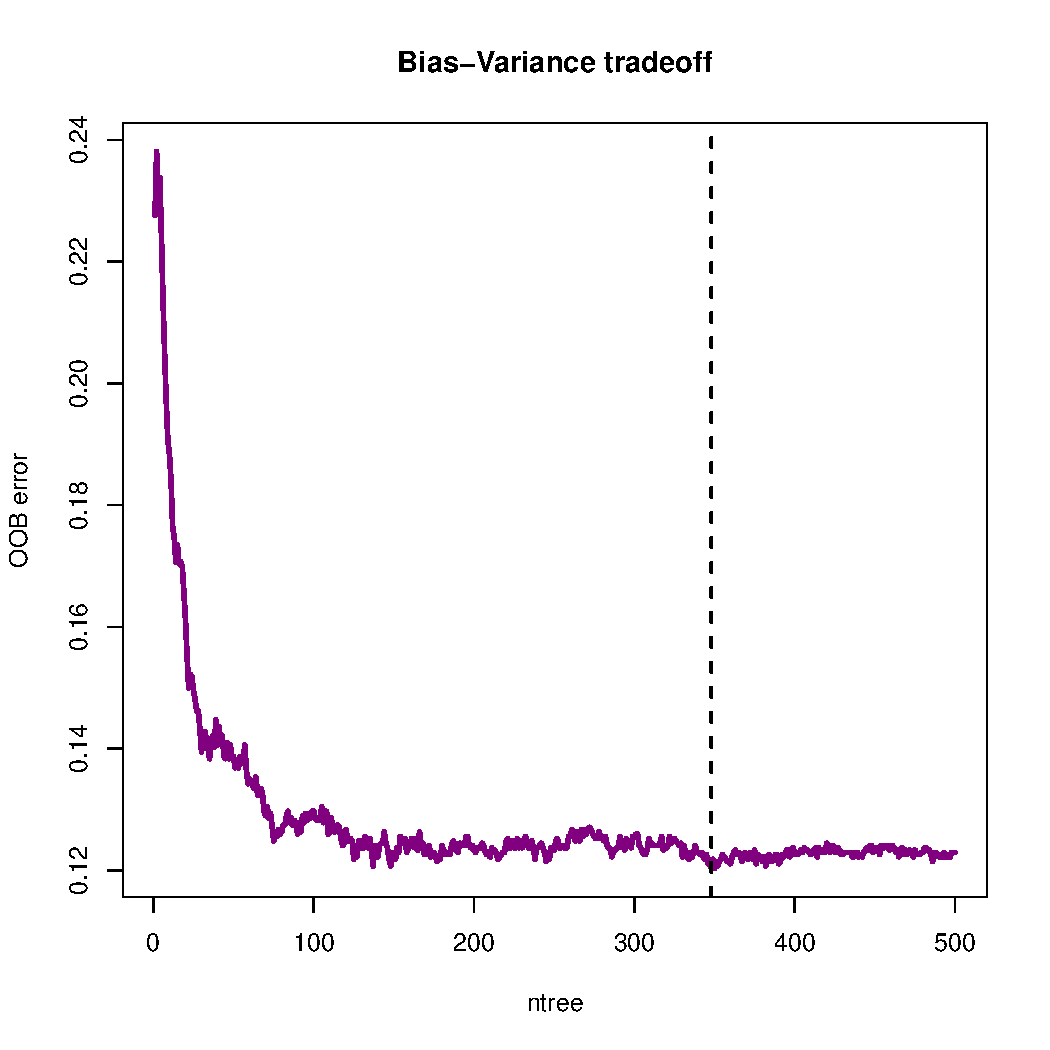
\includegraphics[width=1.1\columnwidth]{../r-StatsLearn-Exam/src/plots/biasvar-rf-apple}
%
%\end{column}
%\end{columns}
%
%\end{frame}

\begin{frame}{Random forest variable importance}

\begin{center}
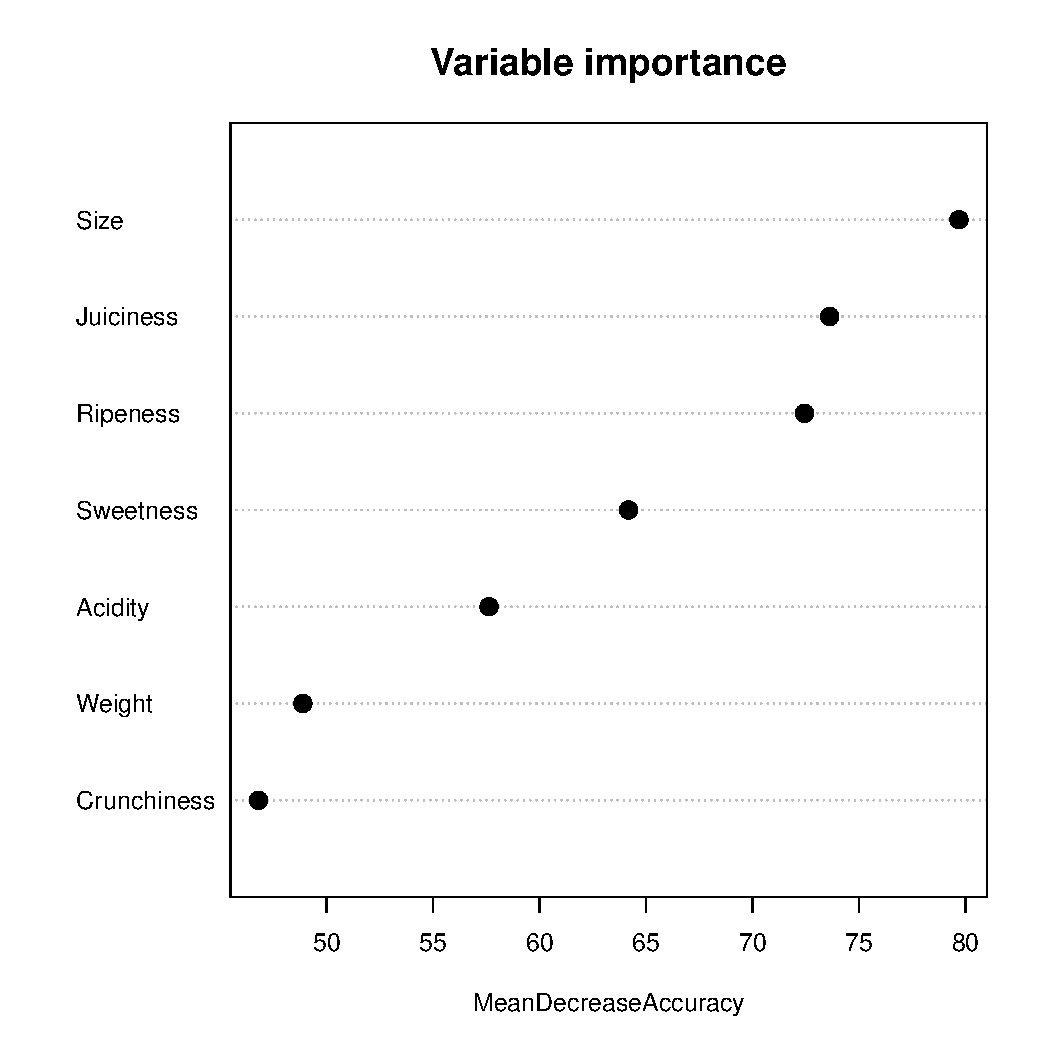
\includegraphics[width=0.7\textwidth]{vip-rf-apple}
\end{center}

\end{frame}

\begin{frame}{AdaBoost variable importance}

\begin{columns}[T]
\hspace*{-3.9em}%
\begin{column}{0.5\textwidth}
	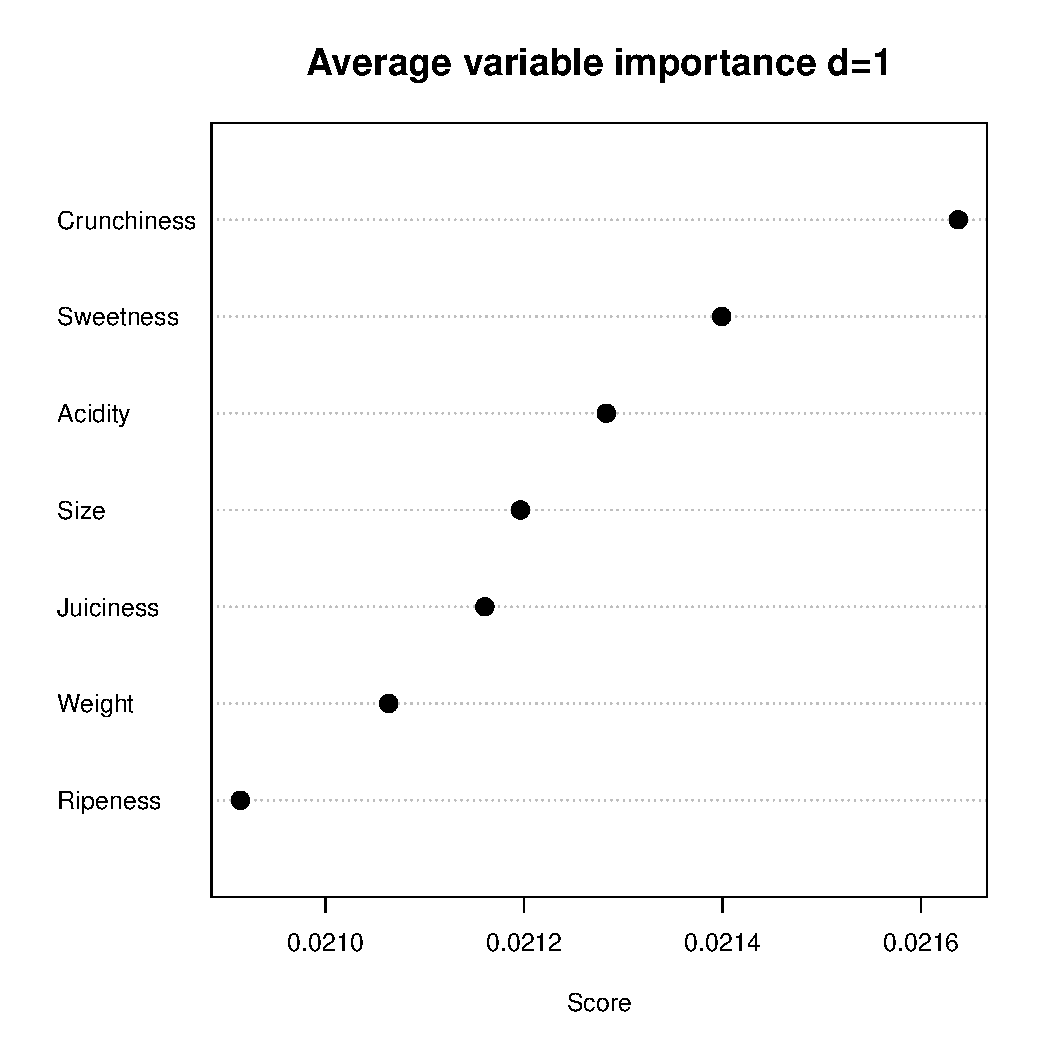
\includegraphics[width=1.25\columnwidth]{vip-ada1-apple}
\end{column}
\hspace*{-1em}%
\begin{column}{0.5\textwidth}
	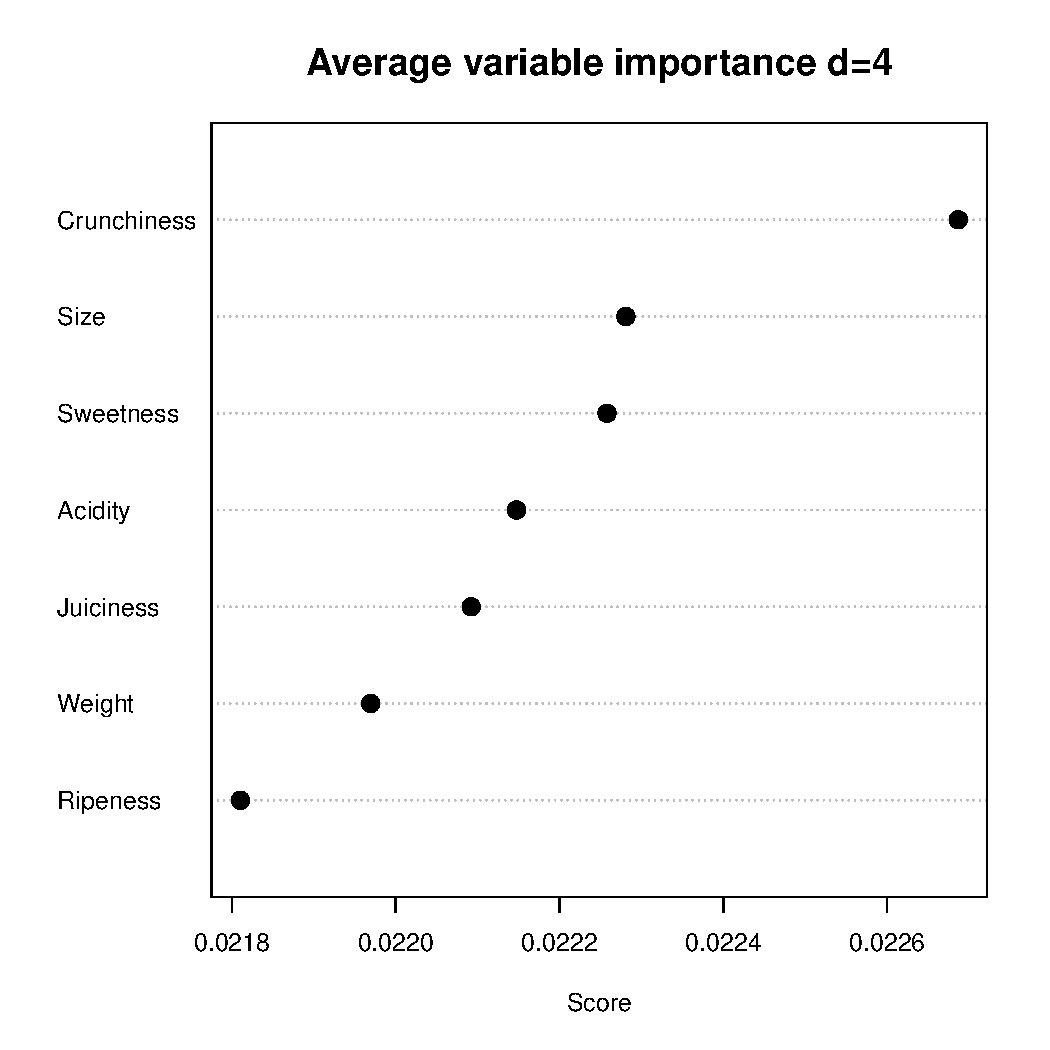
\includegraphics[width=1.25\columnwidth]{vip-ada2-apple}
\end{column}
\end{columns}

\end{frame}

% ------------------------------- %

\begin{frame}[fragile]{Discrete AdaBoost algorithm}
% stochastic setting
% stochastic gradient boosting framework, when bag.frac < 1
% -> shrinkage added
% -> out-of-bag fraction, on each iteration train a classifier on a different dataset sample, keep the rest as OOB

Discrete AdaBoost with shrinkage and out-of-bag, as an additive model with prediction function $f_m(x)$

{%
\setlength{\interspacetitleruled}{0pt}%
\setlength{\algotitleheightrule}{0pt}%
\begin{algorithm}[H]
\KwIn{$M$, $\set{(x_i,y_i)}_1^N$, $x_i\in\R^p$}
%Initialize observation weights $w_i^{(1)}=1/N$ s.t. $\sum_{i=1}^Nw_i^{(m)}=1$\;
Initialize $f_0(x)=0$\;
\For{$m=1$ \KwTo $M$}{
	Set $w_i^{(m)}=-\frac{\partial L(y,g)}{\partial g}\bigr\rvert_{g=f_m(x)}$ s.t.  $\sum_{i=1}^Nw_i^{(m)}=1$\;
	Fit classifier $G_m(x)$ using $w_i^{(m)}$ with samples from $\pi_m$\;
	Weighted error rate $\text{err}_m=\sum_{i=1}^Nw_i^{(m)}\mathbb{I}(y_i\neq G(x_i))$\;
	Set $\alpha_m=\frac{1}{2}\log\bigl(\frac{1-\text{err}_m}{\text{err}_m}\bigr)$\;
	Update $f_{m}(x)\gets f_{m-1}(x)+\lambda\alpha_mG_m(x)$\;
}
\KwOut{$G(x)=\sign(f_M(x))$}
\end{algorithm}}

\end{frame}

% ------------------------------- %

%\begin{frame}{Variable importance comparison}
%
%\begin{columns}[T]
%\hspace*{-4.2em}%
%\begin{column}{0.3\textwidth}
%	\begin{tikzpicture}
%		\tikzset{help lines/.append style=pink}
%%		\draw[help lines] (0,0) grid (5,5); \node[draw,circle,fill=red] at (0,0) {};
%		\node[immagine] (img) at (0,0) {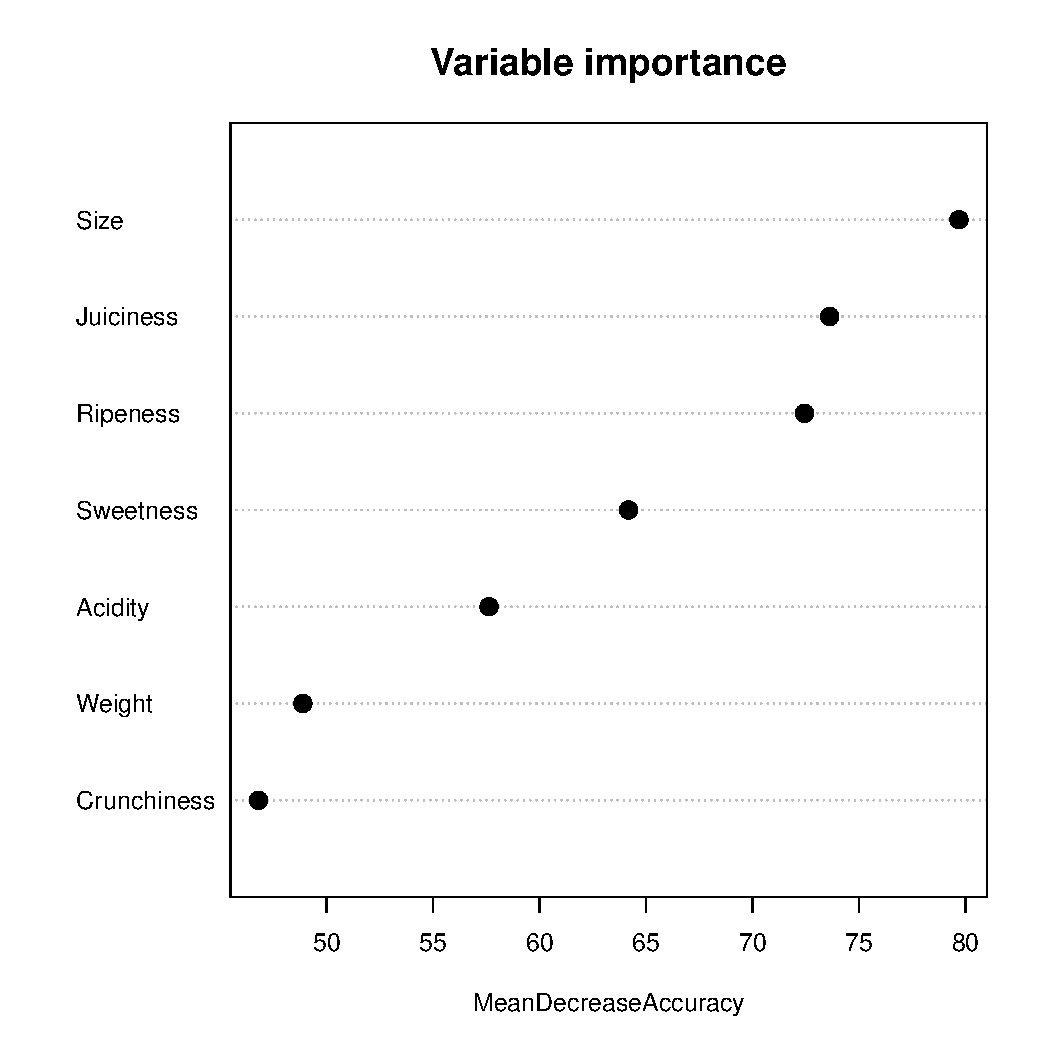
\includegraphics[width=1.475\columnwidth]{vip-rf-apple}};
%		\node[font=\small] at ($(img)+(0,2.8)$) {Random Forest};
%	\end{tikzpicture}
%\end{column}
%\hspace*{-0.7em}%
%\begin{column}{0.3\textwidth}
%	\begin{tikzpicture}
%		\node[immagine] at (0,0) {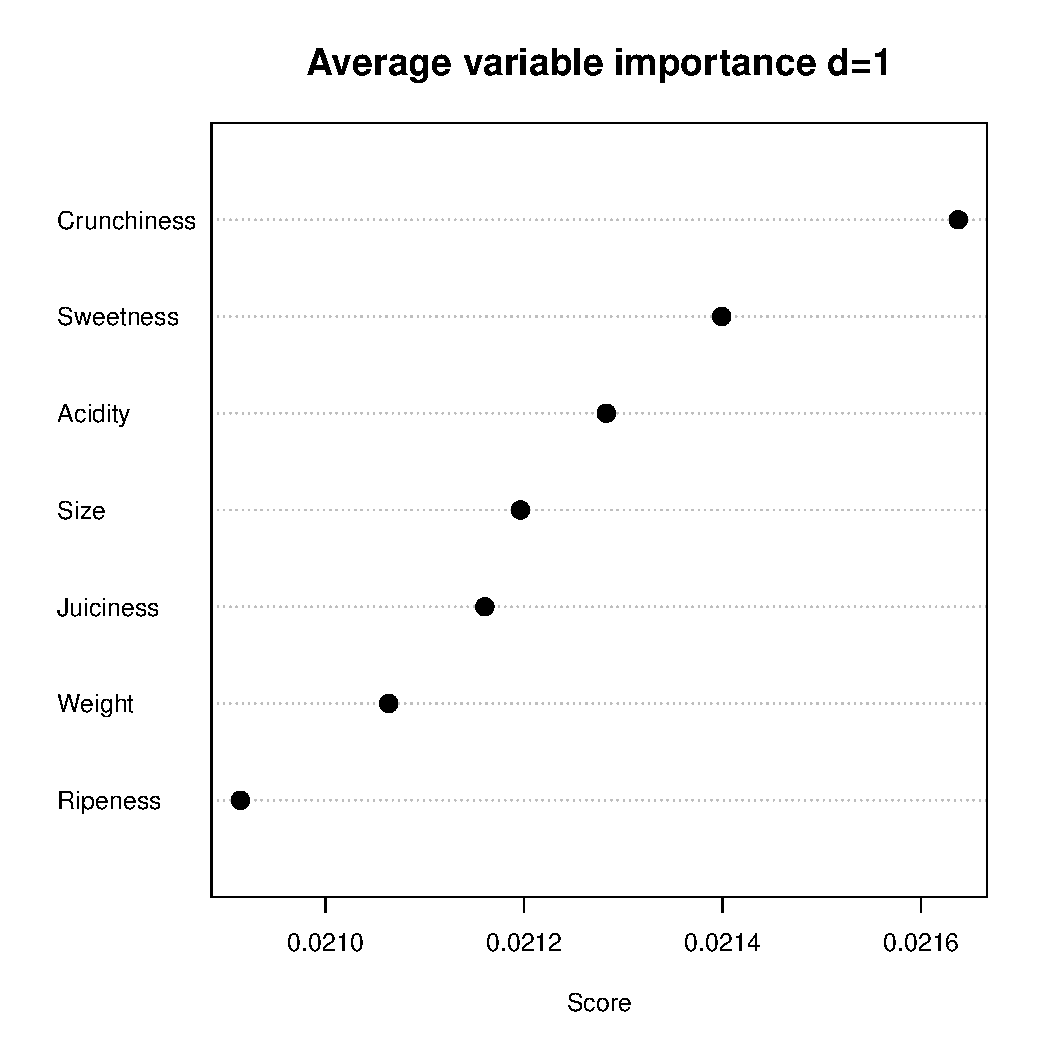
\includegraphics[width=1.475\columnwidth]{vip-ada1-apple}};
%		\node[font=\small] at ($(img)+(0,2.8)$) {$\text{AdaBoost}_{d=1}$};
%	\end{tikzpicture}
%\end{column}
%\hspace*{-0.7em}%
%\begin{column}{0.3\textwidth}
%	\begin{tikzpicture}
%		\node[immagine] at (0,0) {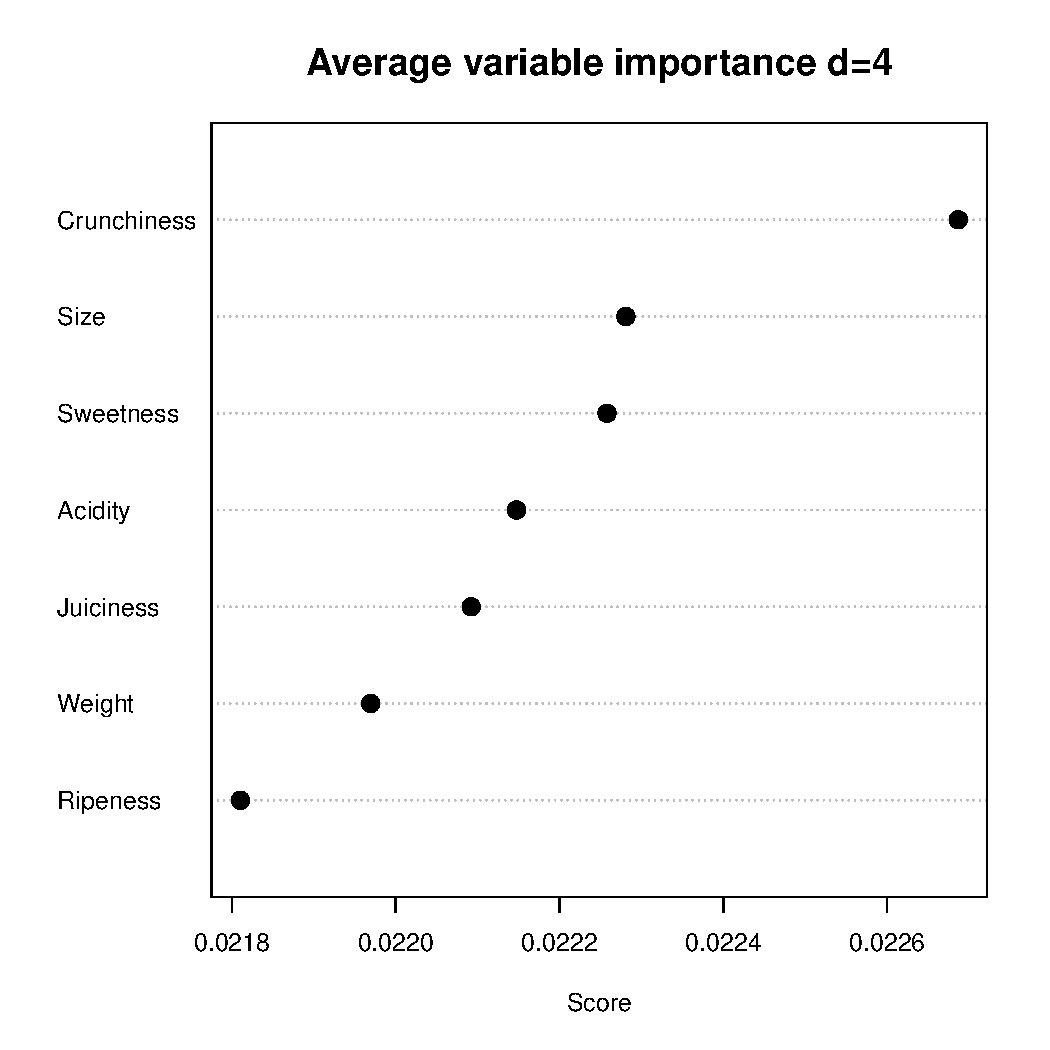
\includegraphics[width=1.475\columnwidth]{vip-ada2-apple}};
%		\node[font=\small] at ($(img)+(0,2.8)$) {$\text{AdaBoost}_{d=4}$};
%	\end{tikzpicture}
%\end{column}
%\end{columns}
%
%\end{frame}

% ------------------------------- %

\begin{frame}{Super Learner algorithm flow diagram}

\begin{figure}
	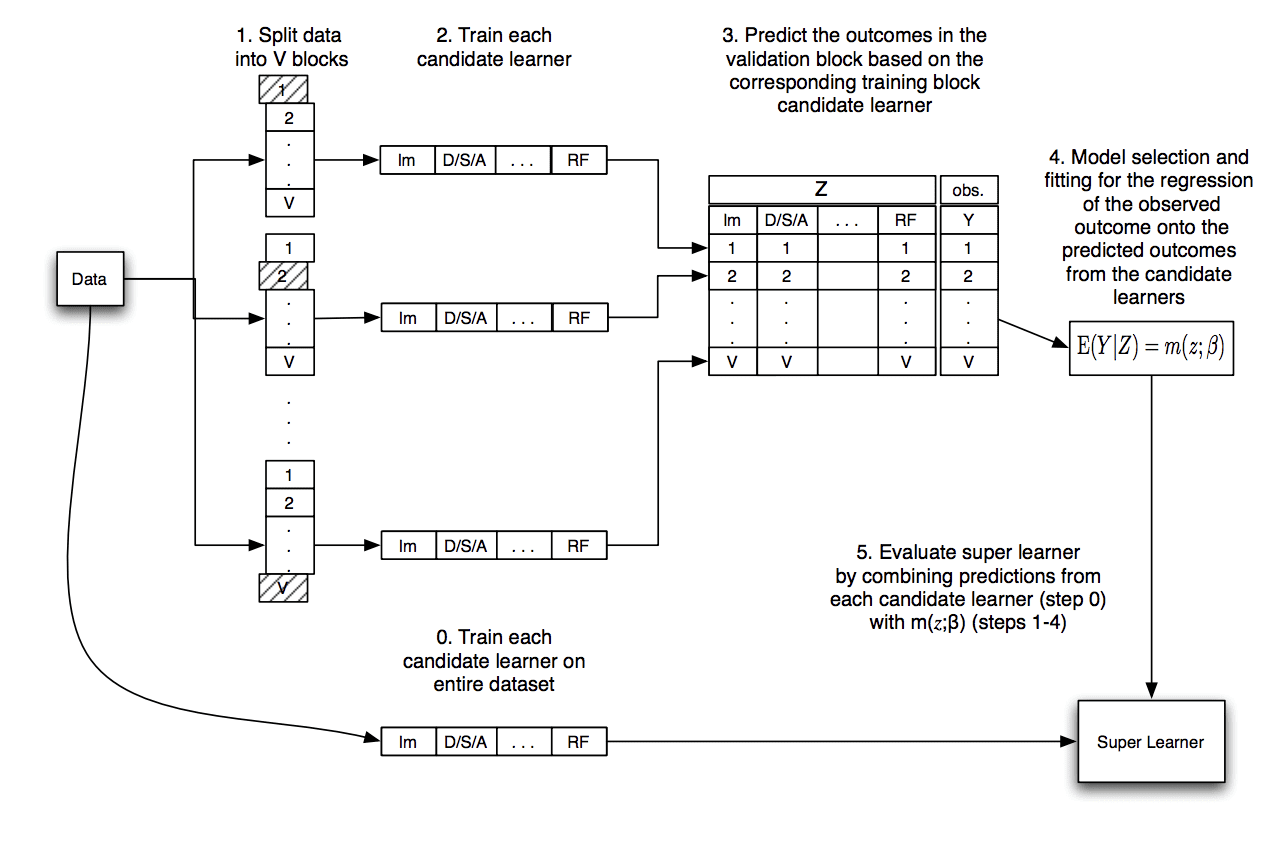
\includegraphics[width=\textwidth]{./Figures/sup-learn.jpg}
\end{figure}

\end{frame}

\begin{frame}[fragile]%{Super learner algorithm}

{%
\setlength{\interspacetitleruled}{0pt}%
\setlength{\algotitleheightrule}{0pt}%
\begin{algorithm}[H]
\KwIn{$\mathcal{D}=\set{(x_i,y_i)}_1^N$, $\mathcal{L}=\set{\phi_k(X)}_{k=1}^K$}
\ForEach{strong learner in $\mathcal{L}$}{%
	Fit $\phi_k$ on $\mathcal{D}$ $\Rightarrow$ $\hat{\phi}_k(\boldsymbol{X})$
	$\rightarrow$ $\hat{\mathcal{L}}=\set{\hat{\phi}_k}_{k=1}^K$\;
}
%Store the fitted library in $\hat{\mathcal{L}}=\set{\hat{\phi}_k(\boldsymbol{X})}_{k=1}^K$\;
\For{$\nu=1,2,\dots,V$}{%
	\ForEach{strong learner in $\mathcal{L}$}{%
		Fit $\phi_k$ on $T(\nu)$, predict $\hat{\phi}_{k,T(\nu)}(X_i\in V(\nu))$\;
	}
}
Stack output in an $N\times K$ matrix
%$Z=\Bigl\{\hat{\phi}_{k,T(\nu)}\bigl(X_{V(\nu)}\bigr),\,\nu=1,2,\dots,V,\,k=1,2,\dots,K\Bigr\}$\;
$Z=\bigl\{\hat{\phi}_{k,T(\nu)}\bigl(X_{V(\nu)}\bigr)\bigr\}$\;
Propose a family of weighted combinations\vspace{-1em}
\[
m(z\rvert\alpha)=\sum_{k=1}^K\alpha_k\hat{\phi}_{k,T(\nu)}\bigl(\boldsymbol{X}_{V(\nu)}\bigr)
\rightarrow
\hat{\alpha}=\argmin_\alpha\sum_{i=1}^NL(Y_i,m(z_i\rvert\alpha))
\vspace*{-1em}\]
of size $N$ s.t. $\alpha_k\geq0$, $\sum_k\alpha_k=1$ and minimizes $\sum_k\alpha_k\hat{\phi}_k$\;
Combine $\hat{\alpha}$ with the library $\hat{\mathcal{L}}$ $\rightarrow$ 
$\hat{\phi}_{\text{SL}}(\boldsymbol{X})=\sum_{k=1}^K\hat{\alpha}_k\hat{\phi}_k(\boldsymbol{X})$\;
\KwOut{$\hat{\phi}_{\text{SL}}$}
\end{algorithm}}

\end{frame}
